\documentclass{article}
%encoding
%--------------------------------------
\usepackage[T1]{fontenc}
\usepackage[utf8]{inputenc}
%--------------------------------------
 
%Portuguese-specific commands
%--------------------------------------
\usepackage[portuguese]{babel}
%--------------------------------------
 
%Hyphenation rules
%--------------------------------------
\usepackage{hyphenat}
\hyphenation{mate-mática recu-perar}
%--------------------------------------


\title{Avaliação da Qualidade de Serviços de Geocodificação Online em Cidades Brasileiras}

\author{Orientador: Prof. Rodrigo Cesar Pedrosa Silva \\
Bolsista: Ana Luiza Almeida Soares}

\date{\today}

\usepackage{natbib}
\usepackage{graphicx}
\usepackage{amsmath}
\usepackage{makecell}
\usepackage{subfigure}

\begin{document}

\maketitle

\section*{Resumo}
Este projeto de pesquisa concentra-se em estimar a qualidade dos serviços de geocodificação online adaptados para cidades brasileiras. A geocodificação, o processo de transformar endereços em coordenadas geográficas, é crucial para uma ampla gama de aplicações em transporte, planejamento urbano, serviços de emergência e operações comerciais. No entanto, a qualidade dos resultados de geocodificação varia entre diferentes provedores de serviço e regiões, tornando necessário avaliar e comparar esses serviços.

O projeto tem como objetivo avaliar a precisão, de diferentes serviços de geocodificação online na correta geocodificação de endereços em cidades brasileiras. Será coletado um conjunto diversificado de dados que incluirá endereços urbanos e rurais com diferentes complexidades. Coordenadas de referência obtidas de fontes confiáveis serão usadas para validar a precisão dos serviços de geocodificação. A pesquisa estabelecerá métricas quantitativas para avaliar e comparar o desempenho dos serviços de geocodificação.

Os resultados deste projeto de pesquisa terão implicações significativas para análise espacial, processos de tomada de decisão, serviços baseados em localização, desenvolvimento de infraestrutura e operações comerciais em cidades brasileiras. Os resultados permitirão que pesquisadores, formuladores de políticas e profissionais tomem decisões informadas sobre a seleção e utilização dos serviços de geocodificação. Além disso, o projeto preenche a lacuna de pesquisa específica para o contexto brasileiro e contribui para o conhecimento existente em pesquisa de geocodificação. Em última análise, este projeto de pesquisa visa aprimorar a precisão, eficiência e confiabilidade dos serviços de geocodificação para cidades brasileiras, beneficiando diversos setores e partes interessadas envolvidas em aplicações de geocodificação.
   
\section*{Palavras-chave}
Geocodificação, Análise espacial, Serviços de geocodificação online
   
\section{Introdução}

\subsection{O problema}
Ao representar locais reais em um computador, é necessário realizar a tradução do endereço (uma sequência de palavras e números) para coordenadas no espaço (latitude e longitude). Esse processo é conhecido como geocodificação. Atualmente, a geocodificação utilizando GeoAPIs online é uma abordagem comum.

No entanto, as GeoAPIs utilizam diferentes métodos para identificar as coordenadas espaciais, e não há garantia de que todas elas sejam precisas. Portanto, é essencial medir a precisão dessas GeoAPIs, a fim de avaliar a qualidade da geocodificação fornecida por cada uma delas.

\subsection{A importância}
A geocodificação de endereços tem aplicações em diversas áreas, tanto dentro quanto fora da computação. A capacidade de mapear um endereço no espaço é crucial para tomadas de decisão, otimização de rotas, planejamento de rotas de fuga, entre outros. É fundamental ter confiança de que os endereços geocodificados realmente representam o local desejado no espaço ou entender quando podem não ser precisos. Isso ajuda a melhorar a confiabilidade do serviço e permite uma tomada de decisão consciente dos riscos envolvidos.

\section{Objetivos}

O objetivo deste estudo é avaliar a qualidade da geocodificação fornecida por cinco GeoAPIs utilizadas no laboratório TerraLAB. As GeoAPIs selecionadas para análise são: TomTom, Mapbox, Open Route Service, Google Maps e Here.
   
\section{Justificativa/Relevância}

As justificativas para este projeto podem ser colocadas nos seguintes termos:

1. Atendendo a uma Necessidade Crítica:

Serviços de geocodificação precisos e confiáveis são essenciais para uma ampla gama de aplicações em diversos setores, incluindo transporte, planejamento urbano, serviços de emergência e operações comerciais \cite{kilic2020accuracy,cortes2021improving}. No contexto das cidades brasileiras, que possuem um sistema de endereçamento complexo e características geográficas diversas, a necessidade de soluções robustas de geocodificação torna-se ainda mais crítica  \cite{martins2012geocodificacao,davis2011evaluation}. Este projeto de pesquisa aborda essa necessidade avaliando e comparando a qualidade de diferentes serviços de geocodificação aplicados à cidades brasileiras.

2. Aprimorando a Análise Espacial e a Tomada de Decisão:

Erros de geocodificação podem ter consequências significativas nos processos de análise espacial e tomada de decisão \cite{cortes2021improving}. Resultados de geocodificação imprecisos ou inexatos podem levar a análises falhas, decisões equivocadas e alocação ineficiente de recursos. Ao estimar a qualidade dos serviços de geocodificação online, este projeto de pesquisa fornece insights valiosos a pesquisadores, formuladores de políticas e profissionais, permitindo que tomem escolhas mais informadas ao utilizar serviços de geocodificação para análises espaciais, planejamento urbano e processos de tomada de decisão.

3. Apoio ao Desenvolvimento de Infraestrutura:

A geocodificação precisa é crucial para iniciativas de desenvolvimento de infraestrutura, incluindo redes de transporte, serviços de utilidade pública e sistemas de resposta a emergências. Ao avaliar a precisão dos serviços de geocodificação, este projeto de pesquisa fornece insights valiosos para planejadores e formuladores de políticas de infraestrutura \cite{de2013deployment}. Os resultados podem contribuir para o desenvolvimento de sistemas de endereçamento robustos, algoritmos de roteamento eficientes e aprimoramento das capacidades de resposta a emergências, aprimorando assim o desenvolvimento geral da infraestrutura nas cidades brasileiras.

4. Preenchendo a Lacuna na Pesquisa:

Embora a pesquisa em geocodificação tenha sido amplamente estudada em vários contextos, há uma falta de avaliações recentes específicas para as cidades brasileiras. Os trabalhos mais atuais são de 2011 e 2012 \cite{davis2011evaluation,martins2012geocodificacao}. Este projeto de pesquisa preenche a lacuna na pesquisa ao se concentrar nos desafios únicos e nos requisitos da geocodificação no contexto brasileiro. Os resultados contribuirão para o conhecimento existente na pesquisa de geocodificação, enriquecendo a compreensão da qualidade e desempenho da geocodificação em sistemas geográficos e de endereçamento diversos.
   
\section{Metodologia}

\subsection{Base de Endereços}
Para avaliar a qualidade das GeoAPIs, utilizaremos uma base de dados confiável que contém endereços completos, tanto verbalmente quanto com suas coordenadas geográficas. Essa base de dados será usada como referência para comparação. Dentro da área, uma base com essas características é chamada de Base Padrão ou Gold Standard Dataset. Sendo assim, iremos nos referir como Base Gold ou Pontos Gold, a base utilizada como referência e os pontos vindos dela.  

A escolha recaiu sobre a base de dados coletada pelo Centro de Estudos da Metrópole (CEM), que inclui mais de 12 mil endereços de escolas na região metropolitana de São Paulo. Essa base foi coletada manualmente por membros do grupo, que visitaram pessoalmente as escolas e utilizaram GPS para obter as coordenadas.

\subsection{Motivo de Escolha da Base de Endereços}
A forma como a base de dados foi coletada é a mais precisa que temos atualmente para obter a localização espacial real de cada endereço. Embora possa haver algum erro devido à precisão do GPS, não existe uma técnica comprovadamente mais eficaz para identificar dados geográficos de um endereço do que a coleta manual. Portanto, utilizaremos essa base como referência, considerando-a o ponto de referência mais próximo da verdadeira localização terrestre. Ao considerar essa base como a correta, poderemos quantificar o erro e calcular métricas com base nisso.

\subsection{Processo de Geocodificação}

\begin{description}
    \item [Seleção dos campos relevantes da base de dados:] A partir da base de dados selecionada, foram identificados os campos que contêm informações sobre o nome da rua, número, bairro, CEP e cidade.
    \item [Homogeneização dos dados:] Os dados obtidos passaram por um processo de homogeneização, no qual foram removidas abreviações comumente utilizadas. Para garantir melhores respostas das GeoAPIs, a equipe decidiu substituir abreviações por suas versões completas. Foi criado um dicionário de abreviações contendo as palavras mais comuns em português e suas formas completas correspondentes. O algoritmo percorre a base de dados e substitui as abreviações encontradas pelas formas completas correspondentes.
    \item [Inserção dos endereços no banco de dados do Crawler:] Os endereços, já homogeneizados, são inseridos no banco de dados do Crawler, que foi desenvolvido pela equipe de Back-end do TerraLAB.
    \item [Realização da geocodificação:] O banco de dados do Crawler é utilizado para realizar a geocodificação dos endereços. A geocodificação consiste em atribuir coordenadas geográficas (latitude e longitude) a cada endereço.O processo de geocodificação é executado utilizando as ferramentas disponíveis no Crawler.
    \item [Armazenamento dos endereços geocodificados:] 
    Os endereços geocodificados são salvos no banco de dados, juntamente com suas coordenadas geográficas.
\end{description}

\begin{figure}[h]
    \centering
    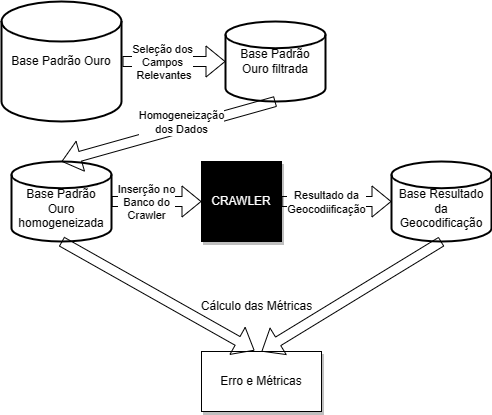
\includegraphics[width=0.5\textwidth]{diagrama monografia.drawio.png}
    \caption{Diagrama que esquematiza os processos necessários para a pesquisa}
    \label{fig:diagramaGeo}
  \end{figure}

\subsection{Metrícas de Avaliação}
A principal métrica utilizada para avaliar a qualidade da geocodificação é o erro do endereço. Esse erro é calculado como a distância entre o ponto gold e o ponto geocodificado pela GeoAPI. Como os pontos estão representados com latitude e longitude, foi utilizada a função distance da biblioteca geopy de python.

\begin{equation}
  e = D(p_{\text{Gold}}, p_{\text{Geo}})
  \end{equation}
  
  onde:
  \begin{itemize}
    \item $e$ é o erro da geocodificação,
    \item $D$ é uma função que calcula a distância em km,
    \item $p_{\text{Gold}}$ é o ponto da base Gold, e
    \item $p_{\text{Geo}}$ é o ponto resultante da geocodificação.
  \end{itemize}

Com base nesse erro, calcularemos medidas estatísticas, como a média, a mediana, o desvio padrão e a média aparada em 5\%, para analisar a precisão das GeoAPIs.

Outra métrica utilizada é a taxa de resposta por API. Para alguns endereços da base de dados, as GeoAPIs podem retornar um erro, não fornecendo uma geocodificação válida. Nesse caso, nada é inserido no banco de dados. A taxa de resposta é calculada como a quantidade de endereços geocodificados dividida pela quantidade de endereços originais na base de dados. Esse valor, normalmente entre 0 e 1, é convertido em uma porcentagem para facilitar a compreensão dos resultados.

\begin{equation}
  \text{tx}_{\text{Resp}} = \frac{n_{\text{Geo}} \times 100}{n_{\text{Gold}}}
  \end{equation}
  
  onde:
  \begin{itemize}
    \item $\text{T}_{\text{Resp}}$ é a taxa de resposta da API,
    \item $n_{\text{Geo}}$ é a quantidade de endereços geocodificados em determinada API, e
    \item $n_{\text{Gold}}$ é a quantidade de endereços da base gold que foram inseridos para geocodificação.
  \end{itemize}
  
\section{Resultados Preliminares}

\subsection{Distribuição Espacial dos Pontos Geocodificados}
Para melhor visualização dos pontos geocodificados em comparação com o banco de referência, foram gerados mapas com a identificação dos pontos para cada uma das APIs. Seguem os mapas. 

\begin{figure}[h]
  \centering
  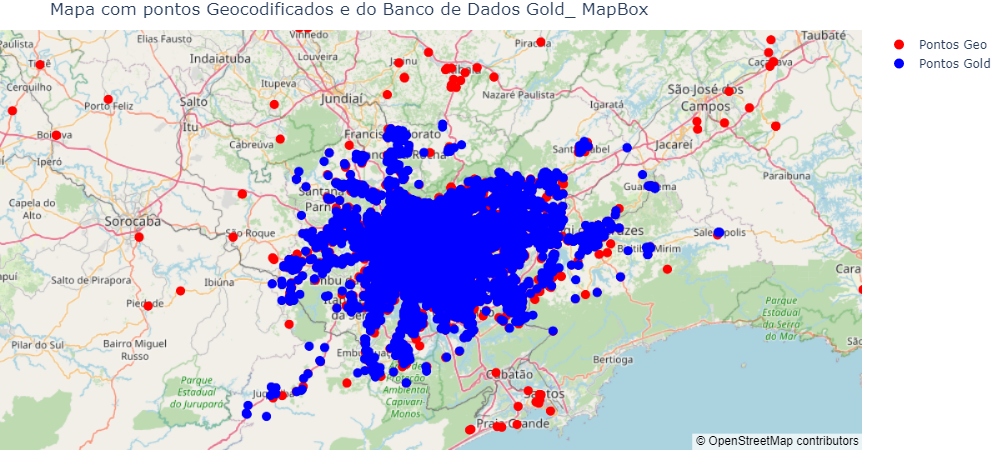
\includegraphics[width=\textwidth]{mapapontos1.png}
  \caption{Mapa da Distribuição Espacial dos Pontos da base Gold e Geocodificados pela Mapbox}
  \label{fig:mapapontos1}
\end{figure}

\begin{figure}[h]
  \centering
  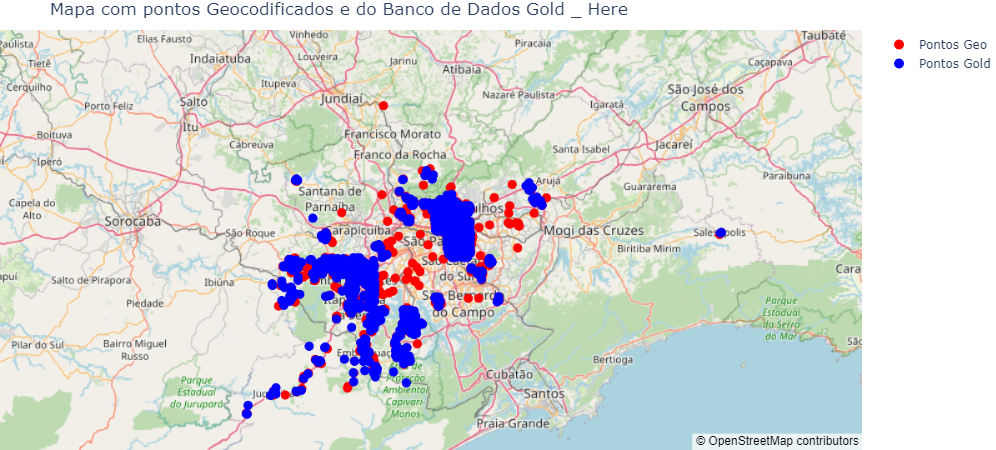
\includegraphics[width=\textwidth]{mapapontos2.png}
  \caption{Mapa da Distribuição Espacial dos Pontos da base Gold e Geocodificados pela Here}
  \label{fig:mapapontos2}
\end{figure}

\begin{figure}[h]
  \centering
  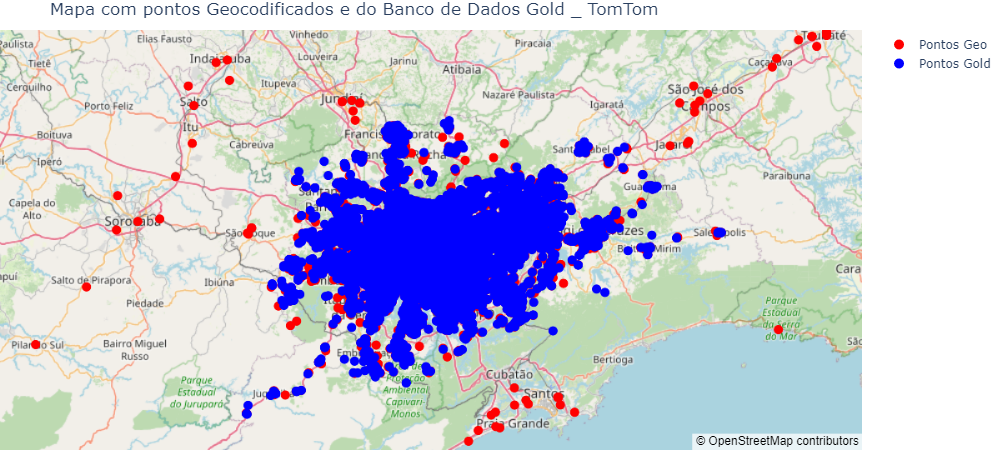
\includegraphics[width=\textwidth]{mapapontos3.png}
  \caption{Mapa da Distribuição Espacial dos Pontos da base Gold e Geocodificados pela TomTom}
  \label{fig:mapapontos3}
\end{figure}

Não é possível tirar muitas conclusões definitivas apenas com essa visualização, no entanto, é possível observar a densidade dos pontos e identificar quais GeoAPIs processaram a maior quantidade de pontos. Além disso, pode-se notar que os pontos classificados como "Gold" estão concentrados na região metropolitana de São Paulo, enquanto alguns pontos geocodificados estão localizados fora dessa região, em outras cidades do estado. Essa disparidade provavelmente reflete alguns erros de geocodificação, conhecidos como outliers.

\subsection{Metrícas do Erro}
Após essa análise, o erro foi calculado para cada um dos pontos, sendo expresso em quilômetros.

Com essa informação, foram calculadas as métricas mencionadas anteriormente. É notável que a API TomTom obteve a maior taxa de resposta, com um índice superior a 80\%. Além disso, apresentou a melhor média aparada em 5\%. Por outro lado, a API Here obteve um desempenho superior na média tradicional, apesar de possuir uma taxa de resposta muito baixa. De forma geral, esses resultados foram considerados insatisfatórios. Ao longo do relatório, iremos analisar outras questões em detalhes.

\begin{table}
  \centering
  \caption{Métricas de Erro e Resposta}
  \setlength{\tabcolsep}{4pt}
  \begin{tabular}{|c|c|c|c|c|c|c|}
  \hline
  \makecell{API} & \makecell{Média \\(km)} & \makecell{Mediana \\(km)} & \makecell{Desvio \\Padrão (km)} & \makecell{Média \\Aparada (km)}(km) & \makecell{Taxa de \\Resposta (\%)} & \makecell{Taxa de \\Acerto(\%)}\\
  \hline
  Mapbox & 9.7544 & 0.1084 & 46.7664 & 1.8349 & 53.3829 & 30.1903 \\
  Tomtom & 5.0701 & 0.0560 & 35.6215 & 0.2373 & 83.1894 & 9.2051 \\
  Here & 2.2372 & 0.0632 & 13.7984 & 0.4365 & 13.9075 & 9.2051 \\
  \hline
  \end{tabular}
\end{table}

\subsection{Distribuição do Erro}
Em seguida, tentamos analisar a distribuição do erro para cada uma das GeoAPIs. Para isso, utilizamos histogramas de erro individualmente para cada API e combinando todas elas. No entanto, devido à presença de alguns erros exorbitantes, esses histogramas não eram muito representativos, pois a maior parte do erro se concentrava entre 0 km e 50 km. Diante disso, decidimos realizar um corte nos dados, limitando o erro em 0.5 km ou 500 metros. Em seguida, repetimos o processo, agora gerando um único histograma que representa a distribuição do erro para todas as APIs em conjunto.

Com base nos histogramas, pudemos observar que a maioria dos erros está concentrada entre 0 e 200 metros. Levando em consideração nossas pesquisas, consideramos um erro aceitável de até 150 metros, o que corresponde aproximadamente a um quarteirão. Portanto, com base apenas na análise da distribuição de erros, todas as APIs apresentam resultados satisfatórios.

\begin{figure}[h]
  \centering
  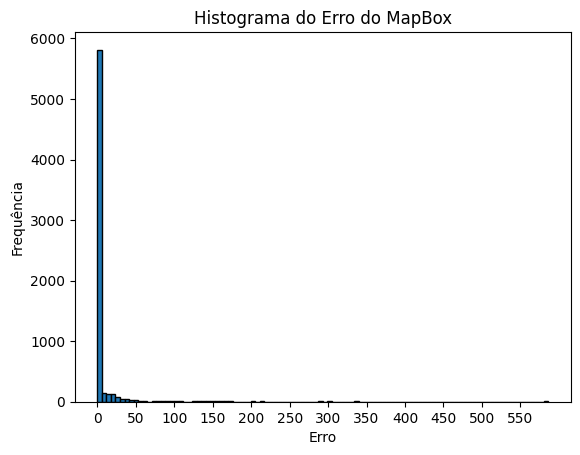
\includegraphics[width=\textwidth]{hist1.png}
  \caption{Histograma do erro calculado com os pontos da Mapbox}
  \label{fig:hist1}
\end{figure}

\begin{figure}[h]
  \centering
  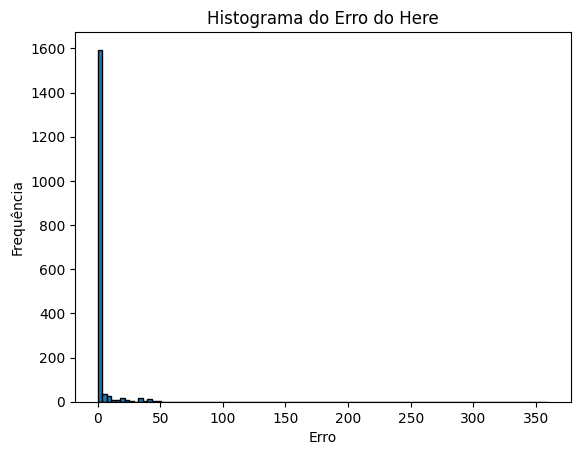
\includegraphics[width=\textwidth]{hist2.png}
  \caption{Histograma do erro calculado com os pontos da Here}
  \label{fig:hist2}
\end{figure}

\begin{figure}[h]
  \centering
  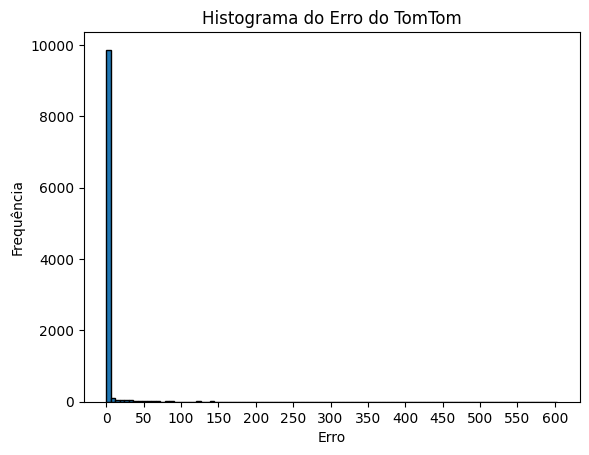
\includegraphics[width=\textwidth]{hist3.png}
  \caption{Histograma do erro calculado com os pontos da TomTom}
  \label{fig:hist3}
\end{figure}

\begin{figure}[h]
  \centering
  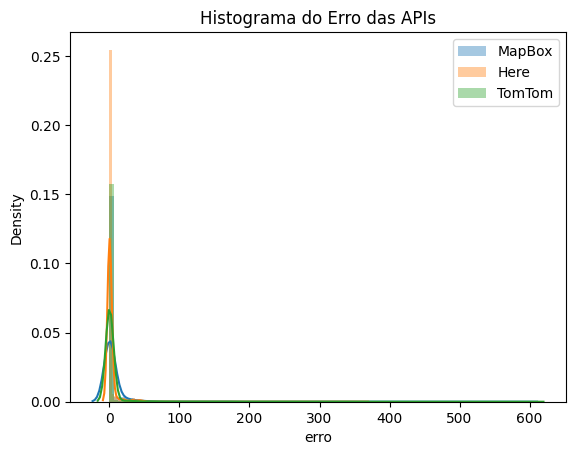
\includegraphics[width=\textwidth]{hist4.png}
  \caption{Histograma comparativo do erro das APIs}
  \label{fig:hist4}
\end{figure}

\begin{figure}[h]
  \centering
  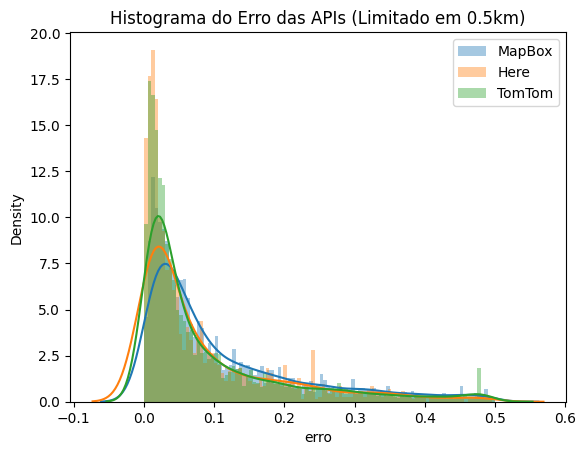
\includegraphics[width=\textwidth]{hist5.png}
  \caption{Histograma comparativo do erro das APIs com limitação em 500 metros}
  \label{fig:hist5}
\end{figure}

\subsection{Distribuição Espacial do Erro}
Além disso, realizamos uma análise adicional para visualizar como esse erro se comporta no espaço. Para isso, criamos mapas de altitude, onde o erro foi utilizado como medida de altitude. Nessa representação, cores mais próximas do vermelho indicam erros mais altos, enquanto cores mais próximas do azul escuro indicam erros mais baixos. Também plotamos os pontos geocodificados no mapa para avaliar a representatividade das cores. Dessa forma, pudemos verificar se uma determinada área apresenta muitos pontos geocodificados ou se há poucos pontos com erros grandes.

Ao analisar os resultados, observamos que a maioria do mapa apresenta erros menores que 34 km, conforme esperado. No entanto, identificamos alguns pontos com erros grandes, que serão avaliados individualmente posteriormente. É importante ressaltar que encontramos uma limitação devido à presença de erros exorbitantes, ou outliers, o que restringe nossa capacidade de tirar conclusões significativas. Para obter uma melhor compreensão do contraste e da distribuição geográfica do erro, planejamos repetir o experimento realizando um corte em 34 km.

É válido destacar que o mapa é interativo no projeto original, permitindo uma visualização mais detalhada das informações apresentadas.

\begin{figure}[h]
  \centering
  \subfigure[Mapa]{
    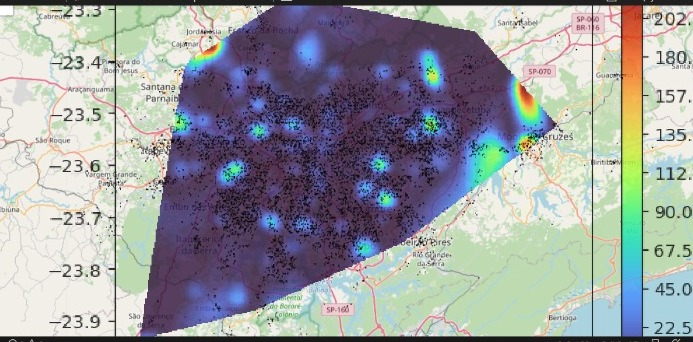
\includegraphics[width=0.45\textwidth]{Mapa.jpeg}
  }
  \subfigure[Gráfico de altitude]{
    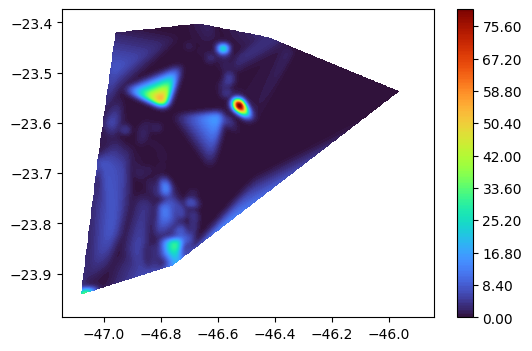
\includegraphics[width=0.45\textwidth]{graficoAltHere.png}
  }
  \caption{Mapa e gráfico de altitude, considerando o erro da Here como a medida de altitude}
  \label{fig:alt1}
\end{figure}

\begin{figure}[h]
  \centering
  \subfigure[Mapa]{
    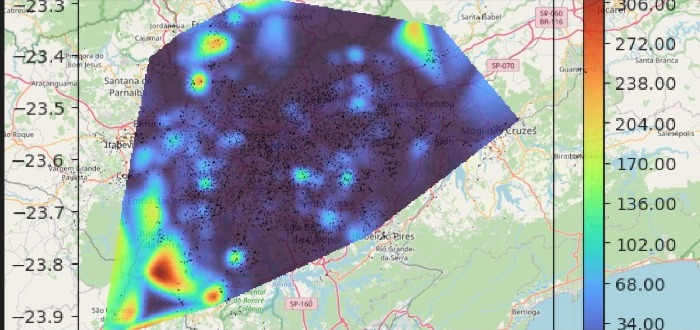
\includegraphics[width=0.45\textwidth]{MapaHere.jpeg}
  }
  \subfigure[Gráfico de altitude]{
    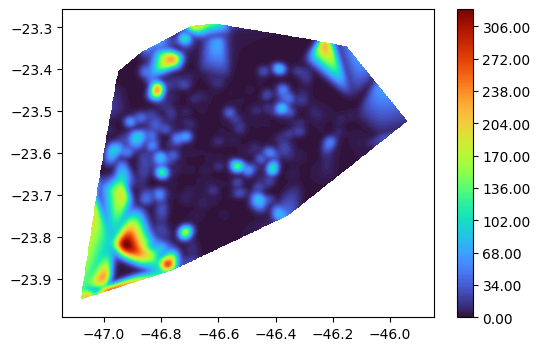
\includegraphics[width=0.45\textwidth]{graficoAltMapbox.png}
  }
  \caption{Mapa e gráfico de altitude, considerando o erro da Mapbox como a medida de altitude}
  \label{fig:alt2}
\end{figure}

\begin{figure}[h]
  \centering
  \subfigure[Mapa]{
    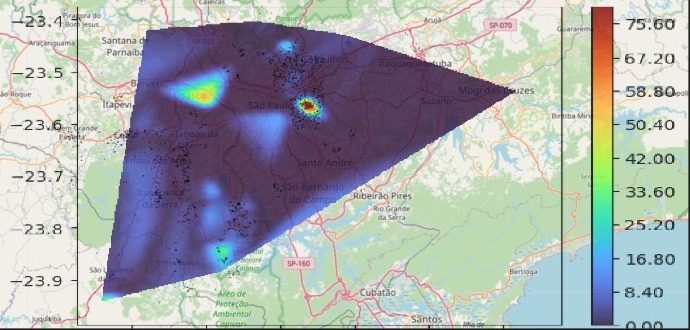
\includegraphics[width=0.45\textwidth]{Mapatomtom.jpeg}
  }
  \subfigure[Gráfico de altitude]{
    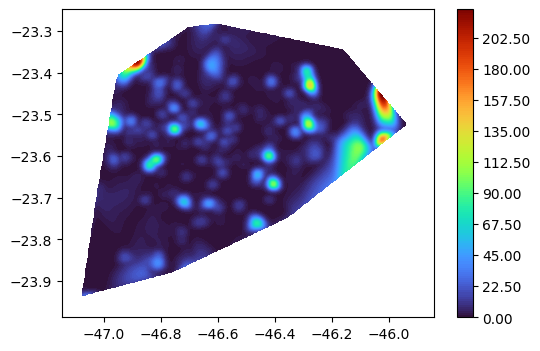
\includegraphics[width=0.45\textwidth]{graficoAltTomtom.png}
  }
  \caption{Mapa e gráfico de altitude, considerando o erro da TomTom como a medida de altitude}
  \label{fig:alt3}
\end{figure}
%(Apenas em caso de renovação)
%(Limite 1500 caracteres)	
   
 

\bibliographystyle{plain}
\bibliography{references}
\end{document}
